\paragraph{Упаковка моделей}

Финальным шагом обработки информационных моделей является упаковка.
Для этого был выбран механизм фреймворка Unity называющийся AssetBundle.
AssetBundle это архив, содержащий не скриптовые ресурсы,
например модели или текстуры, который можно динамически загружать
или выгружать в момент выполнения приложения.
Пакеты могут обладать взаимными зависимостями, например графический материал,
упакованный в один AssetBundle может использовать текстуру,
упакованную в другой AssetBundle (рисунок~\ref{figure:AssetBundleDependency}),
что может сильно уменьшить расход памяти, если таких пакетов
с графическими материалами станет несколько.%
\cite{DocUnity,UnityAssetsResourcesBundles}

\begin{figure}[ht]
    \centering
    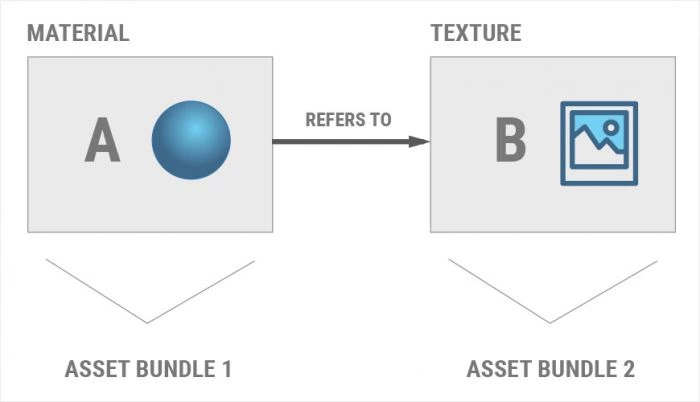
\includegraphics[width=0.8\textwidth]{images/AssetBundleDependency.png}
    \caption{Взаимозависимости ресурсных пакетов.%
    \cite{UnityAssetsResourcesBundles}}
    \label{figure:AssetBundleDependency}
\end{figure}

Помимо этого AssetBundle обладает встроенными механизмами сжатия,
а также механизмами версионности и кеширования,
что позволит эффективнее справляться с модификациями информационной модели.%
\cite{DocUnity,UnityAssetsResourcesBundles}
Создание ресурсных пакетов тоже может быть полностью автоматическим,
что показано на рисунке~\ref{figure:SExportBundles}.

\begin{figure}[ht]
    \centering
    \includegraphics[width=0.6\textwidth]{example-image}
    \caption{Экспорт пакетов}
    \label{figure:SExportBundles}
    \comment{ModelImport.ExportAssetBundles}
\end{figure}

\intextcomment{
    Описание UML-схемы...
}

\comment{
    TODO:

    Запилить UML!

    скрипты смотреть тут
        C:\Users\Egor\Rubius\model-import-test\Assets\Scripts\ModelImport\Editor
}
